\documentclass[11pt]{article}
\usepackage{graphicx}	
\usepackage{amsmath}
\usepackage[margin=1in]{geometry}

\title{Team Project Outline in LaTeX Template}
\author{Ratislav Krylov \and Caleb Lewis}

\begin{document}
\maketitle

\begin{abstract}
This is our abstract wooooo
\end{abstract}

\section{Introduction}
this is an introduction

\section{Methods in this study}
We will now describe each method that we used for this exploration.

\subsection{Euler}
Euler

\subsection{Modified Euler}
Modified Euler

\subsection{Runge-Kutta}
Rk2 and RK4 and Adaptive step stize RK4

\subsection{Adams-Bashforth 4-Step Explicit}


\subsection{Predictor-Corrector Using Adams-Bashforth 4-Step Explicit and Adams-Moulton 3-Step Implicit}
Regular and Adaptive step stize

\section{Numerical experiments}
Here, we'll describe each example and how each method compares in regard to their respective error.

\subsection{Example 1}
Example 1: $y' = y - t^2 + 1$

\subsection{Example 2}
\begin{equation}\label{ex:2:ivp}
y{'} = \frac{1}{t^2} - \frac{y}{t} - y^2, t \in [1,2], y(0) = -1, h = .05
\end{equation}

Exact solution:
\begin{equation}\label{ex:2:ivp}
y(t) = \frac{-1}{t}
\end{equation}
\begin{figure}
\centering
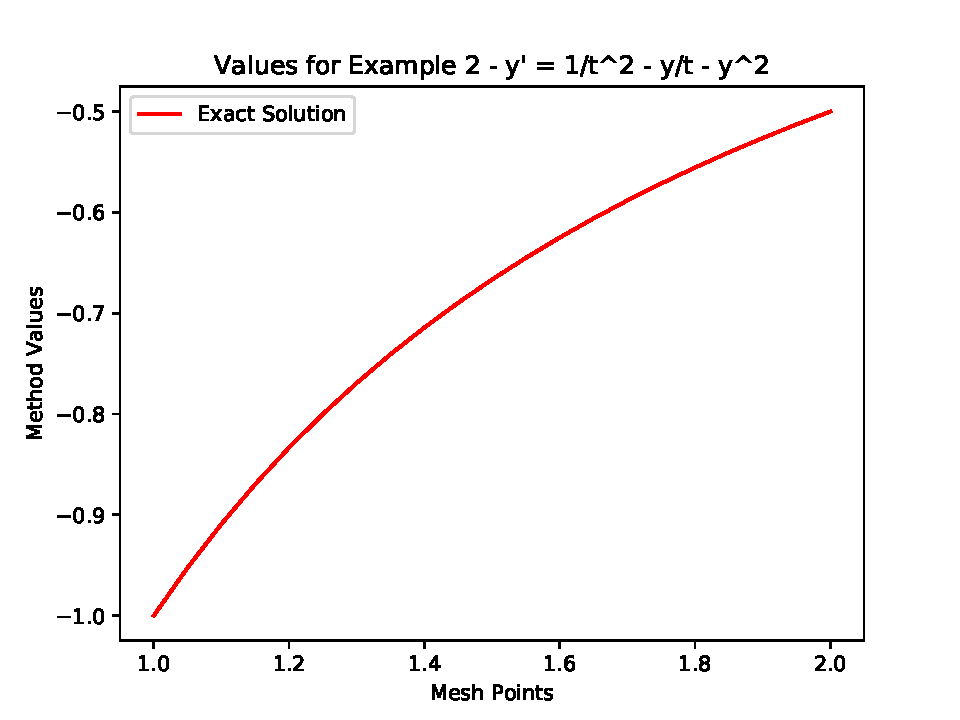
\includegraphics[width=.5\textwidth]{exact_solution_example_2.pdf}
\caption{This is the exact solution to $y(t)=\frac{-1}{t}$}
\label{fig:ex:2:solution}
$rf$
\end{figure}


\subsection{Example 3}
Example 3: 
$z = dy/dt = e^2t * sin(t) - 2y - dz/dx , dz/dt = e^2t * sin(t) + z - 2y$


\subsection{Example 4}
$Example 4: y' = y - t^2 + 1$

\end{document}